\section{Addition Results}
\label{appen:results}

\subsection{Progression Problem 2}
\begin{table}[h]
   \caption{\label{tab:diffusion_diffusion_dom_problem2_results} Convergence Rate for Diffusion-Dominated Problem 2  with Absolute Error}
   \centering
    \scalebox{0.85}{
   \begin{tabular}{clllllll}
   \hline
    Solver & Cells & E${}_{\infty}$ Rate & E${}_{1}$ Rate & E${}_{2}$ Rate & E${}_{\infty}$ Error & E${}_{1}$ Error & E${}_{2}$ Error \\
   \hline
   CRAM &   10 & - & - & - & 7.47e-04 & 4.78e-04 & 1.68e-04 \\
   - &   20 & 2.00 & 2.00 & 2.50 & 1.87e-04 & 1.19e-04 & 2.97e-05 \\ 
   - &   40 & 2.00 & 2.00 & 2.50 & 4.69e-05 & 2.99e-05 & 5.24e-06 \\ 
   - &   80 & 2.00 & 2.00 & 2.50 & 1.17e-05 & 7.46e-06 & 9.27e-07 \\ 
   - &  160 & 2.00 & 2.00 & 2.50 & 2.93e-06 & 1.87e-06 & 1.64e-07 \\ 
   - &  320 & 2.00 & 2.00 & 2.50 & 7.33e-07 & 4.67e-07 & 2.90e-08 \\ 
   \hline
   Parabolic &   10 & - & - & - & 7.47e-04 & 4.78e-04 & 1.68e-04 \\
   - &   20 & 2.00 & 2.00 & 2.50 & 1.87e-04 & 1.19e-04 & 2.97e-05 \\ 
   - &   40 & 2.00 & 2.00 & 2.50 & 4.69e-05 & 2.99e-05 & 5.24e-06 \\ 
   - &   80 & 2.00 & 2.00 & 2.50 & 1.17e-05 & 7.46e-06 & 9.27e-07 \\ 
   - &  160 & 2.00 & 2.00 & 2.50 & 2.93e-06 & 1.87e-06 & 1.64e-07 \\ 
   - &  320 & 2.00 & 2.00 & 2.50 & 7.33e-07 & 4.67e-07 & 2.90e-08 \\ 
   \hline
   Hyperbolic &   10 & - & - & - & 7.47e-04 & 4.78e-04 & 1.68e-04 \\
   - &   20 & 2.00 & 2.00 & 2.50 & 1.87e-04 & 1.19e-04 & 2.97e-05 \\ 
   - &   40 & 2.00 & 2.00 & 2.50 & 4.69e-05 & 2.99e-05 & 5.24e-06 \\ 
   - &   80 & 2.00 & 2.00 & 2.50 & 1.17e-05 & 7.46e-06 & 9.27e-07 \\ 
   - &  160 & 2.00 & 2.00 & 2.50 & 2.93e-06 & 1.87e-06 & 1.64e-07 \\ 
   - &  320 & 2.00 & 2.00 & 2.50 & 7.33e-07 & 4.67e-07 & 2.90e-08 \\ 
   \hline
   Pade-method1 &   10 & - & - & - & 7.47e-04 & 4.78e-04 & 1.68e-04 \\
   - &   20 & 2.00 & 2.00 & 2.50 & 1.87e-04 & 1.19e-04 & 2.97e-05 \\ 
   - &   40 & 2.00 & 2.00 & 2.50 & 4.69e-05 & 2.99e-05 & 5.24e-06 \\ 
   - &   80 & 2.00 & 2.00 & 2.50 & 1.17e-05 & 7.46e-06 & 9.27e-07 \\ 
   - &  160 & 2.00 & 2.00 & 2.50 & 2.93e-06 & 1.87e-06 & 1.64e-07 \\ 
   - &  320 & 2.00 & 2.00 & 2.50 & 7.33e-07 & 4.66e-07 & 2.90e-08 \\ 
   \hline
   Pade-method2 &   10 & - & - & - & 7.47e-04 & 4.78e-04 & 1.68e-04 \\
   - &   20 & 2.00 & 2.00 & 2.50 & 1.87e-04 & 1.19e-04 & 2.97e-05 \\ 
   - &   40 & 2.00 & 2.00 & 2.50 & 4.69e-05 & 2.99e-05 & 5.24e-06 \\ 
   - &   80 & 2.00 & 2.00 & 2.50 & 1.17e-05 & 7.46e-06 & 9.27e-07 \\ 
   - &  160 & 2.00 & 2.00 & 2.50 & 2.93e-06 & 1.87e-06 & 1.64e-07 \\ 
   - &  320 & 2.00 & 2.00 & 2.50 & 7.33e-07 & 4.66e-07 & 2.90e-08 \\ 
   \hline
   Taylor &   10 & - & - & - & 7.47e-04 & 4.78e-04 & 1.68e-04 \\
   - &   20 & 2.00 & 2.00 & 2.50 & 1.87e-04 & 1.19e-04 & 2.97e-05 \\ 
   - &   40 & 2.00 & 2.00 & 2.50 & 4.69e-05 & 2.99e-05 & 5.24e-06 \\ 
   - &   80 & 2.00 & 2.00 & 2.50 & 1.17e-05 & 7.46e-06 & 9.27e-07 \\ 
   - &  160 & 2.00 & 2.00 & 2.50 & 2.93e-06 & 1.87e-06 & 1.64e-07 \\ 
   - &  320 & 2.00 & 2.00 & 2.50 & 7.33e-07 & 4.66e-07 & 2.90e-08 \\ 
   \hline
   \end{tabular}
   }
\end{table}

\clearpage

\begin{table}[p]
   \caption{\label{tab:diffusion_reaction_dom_problem2_results} Convergence Rate for Reaction-Dominated Problem 2  with Absolute Error}
   \centering
    \scalebox{0.85}{
   \begin{tabular}{cllllllll}
   \hline
    Solver & Cells & E${}_{\infty}$ Rate & E${}_{1}$ Rate & E${}_{2}$ Rate & E${}_{\infty}$ Error & E${}_{1}$ Error & E${}_{2}$ Error \\
   \hline
   CRAM &   10 & - & - & - & 8.90e-04 & 5.69e-04 & 2.00e-04 \\ 
   - &   20 & 2.00 & 2.00 & 2.50 & 2.23e-04 & 1.42e-04 & 3.53e-05 \\ 
   - &   40 & 2.00 & 2.00 & 2.50 & 5.58e-05 & 3.55e-05 & 6.24e-06 \\ 
   - &   80 & 2.00 & 2.00 & 2.50 & 1.40e-05 & 8.88e-06 & 1.10e-06 \\ 
   - &  160 & 2.00 & 2.00 & 2.50 & 3.49e-06 & 2.22e-06 & 1.95e-07 \\ 
   - &  320 & 2.00 & 2.00 & 2.50 & 8.72e-07 & 5.55e-07 & 3.45e-08 \\ 
   \hline
   Parabolic &   10 & - & - & - & 8.90e-04 & 5.69e-04 & 2.00e-04 \\ 
   - &   20 & 2.00 & 2.00 & 2.50 & 2.23e-04 & 1.42e-04 & 3.53e-05 \\ 
   - &   40 & 2.00 & 2.00 & 2.50 & 5.58e-05 & 3.55e-05 & 6.24e-06 \\ 
   - &   80 & 2.00 & 2.00 & 2.50 & 1.40e-05 & 8.88e-06 & 1.10e-06 \\ 
   - &  160 & 2.00 & 2.00 & 2.50 & 3.49e-06 & 2.22e-06 & 1.95e-07 \\ 
   - &  320 & 2.00 & 2.00 & 2.50 & 8.72e-07 & 5.55e-07 & 3.45e-08 \\ 
   \hline
   Hyperbolic &   10 & - & - & - & 8.90e-04 & 5.69e-04 & 2.00e-04 \\ 
   - &   20 & 2.00 & 2.00 & 2.50 & 2.23e-04 & 1.42e-04 & 3.53e-05 \\ 
   - &   40 & 2.00 & 2.00 & 2.50 & 5.58e-05 & 3.55e-05 & 6.24e-06 \\ 
   - &   80 & 2.00 & 2.00 & 2.50 & 1.40e-05 & 8.88e-06 & 1.10e-06 \\ 
   - &  160 & 2.00 & 2.00 & 2.50 & 3.49e-06 & 2.22e-06 & 1.95e-07 \\ 
   - &  320 & 2.00 & 2.00 & 2.50 & 8.72e-07 & 5.55e-07 & 3.45e-08 \\ 
   \hline
   Pade-method1 &   10 & - & - & - & 8.90e-04 & 5.69e-04 & 2.00e-04 \\ 
   - &   20 & 2.00 & 2.00 & 2.50 & 2.23e-04 & 1.42e-04 & 3.53e-05 \\ 
   - &   40 & 2.00 & 2.00 & 2.50 & 5.58e-05 & 3.55e-05 & 6.24e-06 \\ 
   - &   80 & 2.00 & 2.00 & 2.50 & 1.40e-05 & 8.88e-06 & 1.10e-06 \\ 
   - &  160 & 2.00 & 2.00 & 2.50 & 3.49e-06 & 2.22e-06 & 1.95e-07 \\ 
   - &  320 & 2.00 & 2.00 & 2.50 & 8.72e-07 & 5.55e-07 & 3.45e-08 \\ 
   \hline
   Pade-method2 &   10 & - & - & - & 8.90e-04 & 5.69e-04 & 2.00e-04 \\ 
   - &   20 & 2.00 & 2.00 & 2.50 & 2.23e-04 & 1.42e-04 & 3.53e-05 \\ 
   - &   40 & 2.00 & 2.00 & 2.50 & 5.58e-05 & 3.55e-05 & 6.24e-06 \\ 
   - &   80 & 2.00 & 2.00 & 2.50 & 1.40e-05 & 8.88e-06 & 1.10e-06 \\ 
   - &  160 & 2.00 & 2.00 & 2.50 & 3.49e-06 & 2.22e-06 & 1.95e-07 \\ 
   - &  320 & 2.00 & 2.00 & 2.50 & 8.72e-07 & 5.55e-07 & 3.45e-08 \\ 
   \hline
   Taylor &   10 & - & - & - & 8.90e-04 & 5.69e-04 & 2.00e-04 \\ 
   - &   20 & 2.00 & 2.00 & 2.50 & 2.23e-04 & 1.42e-04 & 3.53e-05 \\ 
   - &   40 & 2.00 & 2.00 & 2.50 & 5.58e-05 & 3.55e-05 & 6.24e-06 \\ 
   - &   80 & 2.00 & 2.00 & 2.50 & 1.40e-05 & 8.88e-06 & 1.10e-06 \\ 
   - &  160 & 2.00 & 2.00 & 2.50 & 3.49e-06 & 2.22e-06 & 1.95e-07 \\ 
   - &  320 & 2.00 & 2.00 & 2.50 & 8.72e-07 & 5.55e-07 & 3.45e-08 \\ 
   \hline
   \end{tabular}
   }
\end{table}

\clearpage

\begin{table}[p]
   \caption{\label{tab:diffusion_stiff_reaction_dom_problem2_results} Convergence Rate for Stiff Reaction-Dominated Problem 2  with Absolute Error}
   \centering
    \scalebox{0.8}{
   \begin{tabular}{cllllllll}
   \hline
    Solver & Cells & E${}_{\infty}$ Rate & E${}_{1}$ Rate & E${}_{2}$ Rate & E${}_{\infty}$ Error & E${}_{1}$ Error & E${}_{2}$ Error \\
   \hline
   CRAM &   10 & - & - & - & 3.76e-02 & 2.40e-02 & 8.43e-03 \\  
   - &   20 & 2.00 & 2.00 & 2.50 & 9.42e-03 & 6.00e-03 & 1.49e-03 \\  
   - &   40 & 2.00 & 2.00 & 2.50 & 2.36e-03 & 1.50e-03 & 2.63e-04 \\  
   - &   80 & 2.00 & 2.00 & 2.50 & 5.89e-04 & 3.75e-04 & 4.66e-05 \\  
   - &  160 & 2.00 & 2.00 & 2.50 & 1.47e-04 & 9.38e-05 & 8.23e-06 \\  
   - &  320 & 2.00 & 2.00 & 2.50 & 3.68e-05 & 2.34e-05 & 1.46e-06 \\  
   \hline
   Parabolic &   10 & - & - & - & 3.76e-02 & 2.40e-02 & 8.43e-03 \\  
   - &   20 & 2.00 & 2.00 & 2.50 & 9.42e-03 & 6.00e-03 & 1.49e-03 \\  
   - &   40 & 2.00 & 2.00 & 2.50 & 2.36e-03 & 1.50e-03 & 2.63e-04 \\  
   - &   80 & 2.00 & 2.00 & 2.50 & 5.89e-04 & 3.75e-04 & 4.66e-05 \\  
   - &  160 & 2.00 & 2.00 & 2.50 & 1.47e-04 & 9.38e-05 & 8.23e-06 \\  
   - &  320 & 2.00 & 2.00 & 2.50 & 3.68e-05 & 2.34e-05 & 1.46e-06 \\  
   \hline
   Hyperbolic &   10 & - & - & - & 3.76e-02 & 2.40e-02 & 8.43e-03 \\  
   - &   20 & 2.00 & 2.00 & 2.50 & 9.42e-03 & 6.00e-03 & 1.49e-03 \\  
   - &   40 & 2.00 & 2.00 & 2.50 & 2.36e-03 & 1.50e-03 & 2.63e-04 \\  
   - &   80 & 2.00 & 2.00 & 2.50 & 5.89e-04 & 3.75e-04 & 4.66e-05 \\  
   - &  160 & 2.00 & 2.00 & 2.50 & 1.47e-04 & 9.38e-05 & 8.23e-06 \\  
   - &  320 & 2.00 & 2.00 & 2.50 & 3.68e-05 & 2.34e-05 & 1.46e-06 \\  
   \hline
   Pade-method1 &   10 & - & - & - & 3.76e-02 & 2.40e-02 & 8.43e-03 \\  
   - &   20 & 2.00 & 2.00 & 2.50 & 9.42e-03 & 6.00e-03 & 1.49e-03 \\  
   - &   40 & 2.00 & 2.00 & 2.50 & 2.36e-03 & 1.50e-03 & 2.63e-04 \\  
   - &   80 & 2.00 & 2.00 & 2.50 & 5.89e-04 & 3.75e-04 & 4.66e-05 \\  
   - &  160 & 2.00 & 2.00 & 2.50 & 1.47e-04 & 9.38e-05 & 8.23e-06 \\  
   - &  320 & 2.00 & 2.00 & 2.50 & 3.68e-05 & 2.34e-05 & 1.46e-06 \\  
   \hline
   Pade-method2 &   10 & - & - & - & 3.76e-02 & 2.40e-02 & 8.43e-03 \\  
   - &   20 & 2.00 & 2.00 & 2.50 & 9.42e-03 & 6.00e-03 & 1.49e-03 \\  
   - &   40 & 2.00 & 2.00 & 2.50 & 2.36e-03 & 1.50e-03 & 2.63e-04 \\  
   - &   80 & 2.00 & 2.00 & 2.50 & 5.89e-04 & 3.75e-04 & 4.66e-05 \\  
   - &  160 & 2.00 & 2.00 & 2.50 & 1.47e-04 & 9.38e-05 & 8.23e-06 \\  
   - &  320 & 2.00 & 2.00 & 2.50 & 3.68e-05 & 2.34e-05 & 1.46e-06 \\  
   \hline
   Taylor &   10 & - & - & - & 3.76e-02 & 2.40e-02 & 8.43e-03 \\  
   - &   20 & 2.00 & 2.00 & 2.50 & 9.42e-03 & 6.00e-03 & 1.49e-03 \\  
   - &   40 & 2.00 & 2.00 & 2.50 & 2.36e-03 & 1.50e-03 & 2.63e-04 \\  
   - &   80 & 2.00 & 2.00 & 2.50 & 5.89e-04 & 3.75e-04 & 4.66e-05 \\  
   - &  160 & 2.00 & 2.00 & 2.50 & 1.47e-04 & 9.38e-05 & 8.23e-06 \\  
   - &  320 & 2.00 & 2.00 & 2.50 & 3.68e-05 & 2.34e-05 & 1.46e-06 \\  
   \hline
   \end{tabular}
   }
\end{table}

\clearpage

\subsection{Progression Problem 4}
\begin{figure}[p]
    \centering
    \includegraphics[width=6in]{images/chapter-5/progressionProblems/problem4/problem4EinfErrorWithSpace.png}
    \caption{Problem 4 absolute E${}_{\infty}$ error with spatial discretization at various time steps }
    \label{fig:problem4_linferror_spatial_results}
\end{figure}

\clearpage

\begin{figure}[p]
    \centering
    \includegraphics[width=6in]{images/chapter-5/progressionProblems/problem4/problem4EinfErrorWithTime.png}
    \caption{Problem 4 absolute E${}_{\infty}$ error with temporal discretization at various number of spatial cells}
    \label{fig:problem4_linferror_time_results}
\end{figure}


\begin{figure}[p]
    \centering
    \includegraphics[width=6in]{images/chapter-5/progressionProblems/problem4/problem4E2ErrorWithSpace.png}
    \caption{Problem 4 absolute E${}_{2}$ error with spatial discretization at various time steps }
    \label{fig:problem4_l2error_spatial_results}
\end{figure}

\clearpage

\begin{figure}[p]
    \centering
    \includegraphics[width=6in]{images/chapter-5/progressionProblems/problem4/problem4E2ErrorWithTime.png}
    \caption{Problem 4 absolute E${}_{2}$ error with temporal discretization at various number of spatial cells}
    \label{fig:problem4_l2error_time_results}
\end{figure}

\clearpage

\begin{figure}[p]
    \centering
    \includegraphics[width=6in]{images/chapter-5/progressionProblems/problem4/problem4EinftyFluxLimiterConvergenceRate.png}
    \caption{Problem 4 flux limiter E${}_{\infty}$ convergence rate using absolute error}
    \label{fig:problem4_linferror_fluxlimiter_convergence_rate}
\end{figure}

\clearpage

\begin{figure}[p]
    \centering
    \includegraphics[width=6in]{images/chapter-5/progressionProblems/problem4/problem4E2FluxLimiterConvergenceRate.png}
    \caption{Problem 4 flux limiter E${}_{2}$ convergence rate using absolute error}
    \label{fig:problem4_l2error_fluxlimiter_convergence_rate}
\end{figure}

\clearpage

\subsection{Progression Problem 5}
\begin{figure}[p]
    \centering
    \includegraphics[width=6in]{images/chapter-5/progressionProblems/problem5/problem5EinfErrorWithSpace.png}
    \caption{Problem 5 relative E${}_{\infty}$ error with spatial discretization at various time steps }
    \label{fig:problem5_linferror_spatial_results}
\end{figure}

\clearpage

\begin{figure}[p]
    \centering
    \includegraphics[width=6in]{images/chapter-5/progressionProblems/problem5/problem5EinfErrorWithTime.png}
    \caption{Problem 5 relative E${}_{\infty}$ error with temporal discretization at various number of spatial cells}
    \label{fig:problem5_linferror_time_results}
\end{figure}


\begin{figure}[p]
    \centering
    \includegraphics[width=6in]{images/chapter-5/progressionProblems/problem5/problem5E2ErrorWithSpace.png}
    \caption{Problem 5 relative E${}_{2}$ error with spatial discretization at various time steps }
    \label{fig:problem5_l2error_spatial_results}
\end{figure}

\clearpage

\begin{figure}[p]
    \centering
    \includegraphics[width=6in]{images/chapter-5/progressionProblems/problem5/problem5E2ErrorWithTime.png}
    \caption{Problem 5 relative E${}_{2}$ error with temporal discretization at various number of spatial cells}
    \label{fig:problem5_l2error_time_results}
\end{figure}

\clearpage

\begin{figure}[p]
    \centering
    \includegraphics[width=6in]{images/chapter-5/progressionProblems/problem5/problem5EinftyFluxLimiterConvergenceRate.png}
    \caption{Problem 5 flux limiter relative E${}_{\infty}$ spatial convergence rate using absolute error}
    \label{fig:problem5_linferror_fluxlimiter_convergence_rate}
\end{figure}

\clearpage

\begin{figure}[p]
    \centering
    \includegraphics[width=6in]{images/chapter-5/progressionProblems/problem5/problem5E2FluxLimiterConvergenceRate.png}
    \caption{Problem 5 flux limiter relative E${}_{2}$ spatial convergence rate using absolute error}
    \label{fig:problem5_l2error_fluxlimiter_convergence_rate}
\end{figure}

\clearpage

\subsection{Progression Problem 6}
\begin{figure}[p]
    \centering
    \includegraphics[width=6in]{images/chapter-5/progressionProblems/problem6/problem6EinfErrorWithSpace.png}
    \caption{Problem 6 relative E${}_{\infty}$ error with spatial discretization at various time steps }
    \label{fig:problem6_linferror_spatial_results}
\end{figure}

\clearpage

\begin{figure}[p]
    \centering
    \includegraphics[width=6in]{images/chapter-5/progressionProblems/problem6/problem6EinfErrorWithTime.png}
    \caption{Problem 6 relative E${}_{\infty}$ error with temporal discretization at various number of spatial cells}
    \label{fig:problem6_linferror_time_results}
\end{figure}


\begin{figure}[p]
    \centering
    \includegraphics[width=6in]{images/chapter-5/progressionProblems/problem6/problem6E2ErrorWithSpace.png}
    \caption{Problem 6 relative E${}_{2}$ error with spatial discretization at various time steps }
    \label{fig:problem6_l2error_spatial_results}
\end{figure}

\clearpage

\begin{figure}[p]
    \centering
    \includegraphics[width=6in]{images/chapter-5/progressionProblems/problem6/problem6E2ErrorWithTime.png}
    \caption{Problem 6 relative E${}_{2}$ error with temporal discretization at various number of spatial cells}
    \label{fig:problem6_l2error_time_results}
\end{figure}

\clearpage

\begin{figure}[p]
    \centering
    \includegraphics[width=6in]{images/chapter-5/progressionProblems/problem6/problem6EinftyFluxLimiterConvergenceRate.png}
    \caption{Problem 6 flux limiter relative E${}_{\infty}$ spatial convergence rate}
    \label{fig:problem6_linferror_fluxlimiter_convergence_rate}
\end{figure}

\clearpage

\begin{figure}[p]
    \centering
    \includegraphics[width=6in]{images/chapter-5/progressionProblems/problem6/problem6E2FluxLimiterConvergenceRate.png}
    \caption{Problem 6 flux limiter relative E${}_{2}$ convergence rate}
    \label{fig:problem6_l2error_fluxlimiter_convergence_rate}
\end{figure}

\clearpage

\subsection{Progression Problem 7}

\begin{figure}[p]
    \centering
    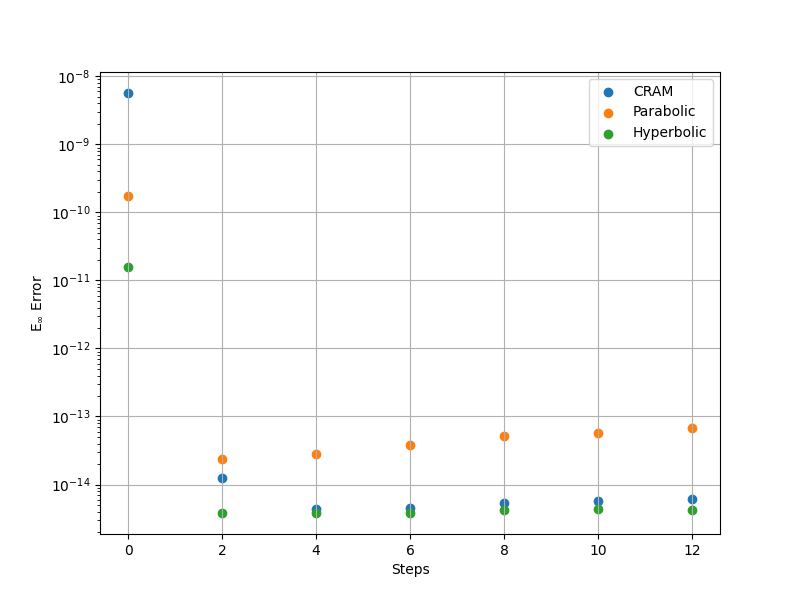
\includegraphics[width=6in]{images/chapter-5/progressionProblems/problem7/problem7EinfErrorWithSteps.png}
    \caption{Problem 7 E${}_{\infty}$ relative error with sub-steps}
    \label{fig:problem7_Einf_error_with_steps}
\end{figure}

\clearpage

\begin{figure}[p]
    \centering
    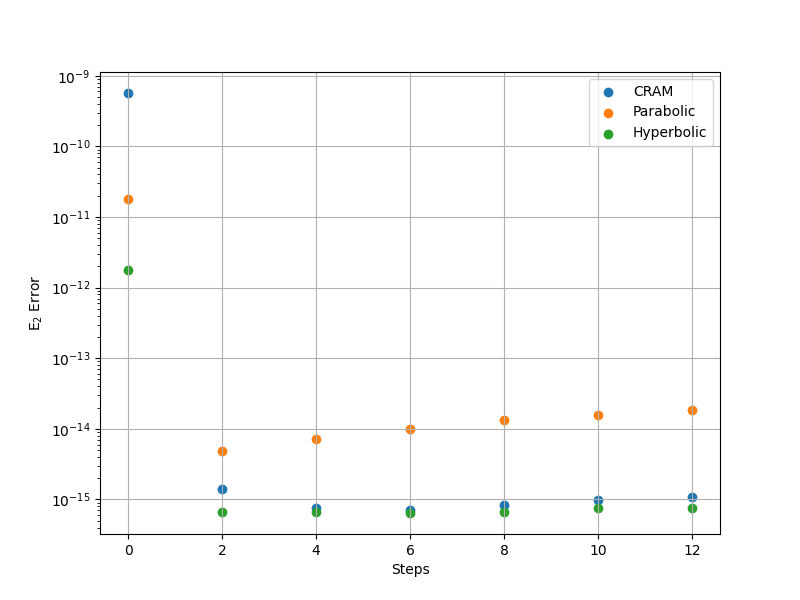
\includegraphics[width=6in]{images/chapter-5/progressionProblems/problem7/problem7E2ErrorWithSteps.png}
    \caption{Problem 7 E${}_{2}$ relative error with sub-steps}
    \label{fig:problem7_E2_error_with_steps}
\end{figure}

\begin{figure}[p]
    \centering
    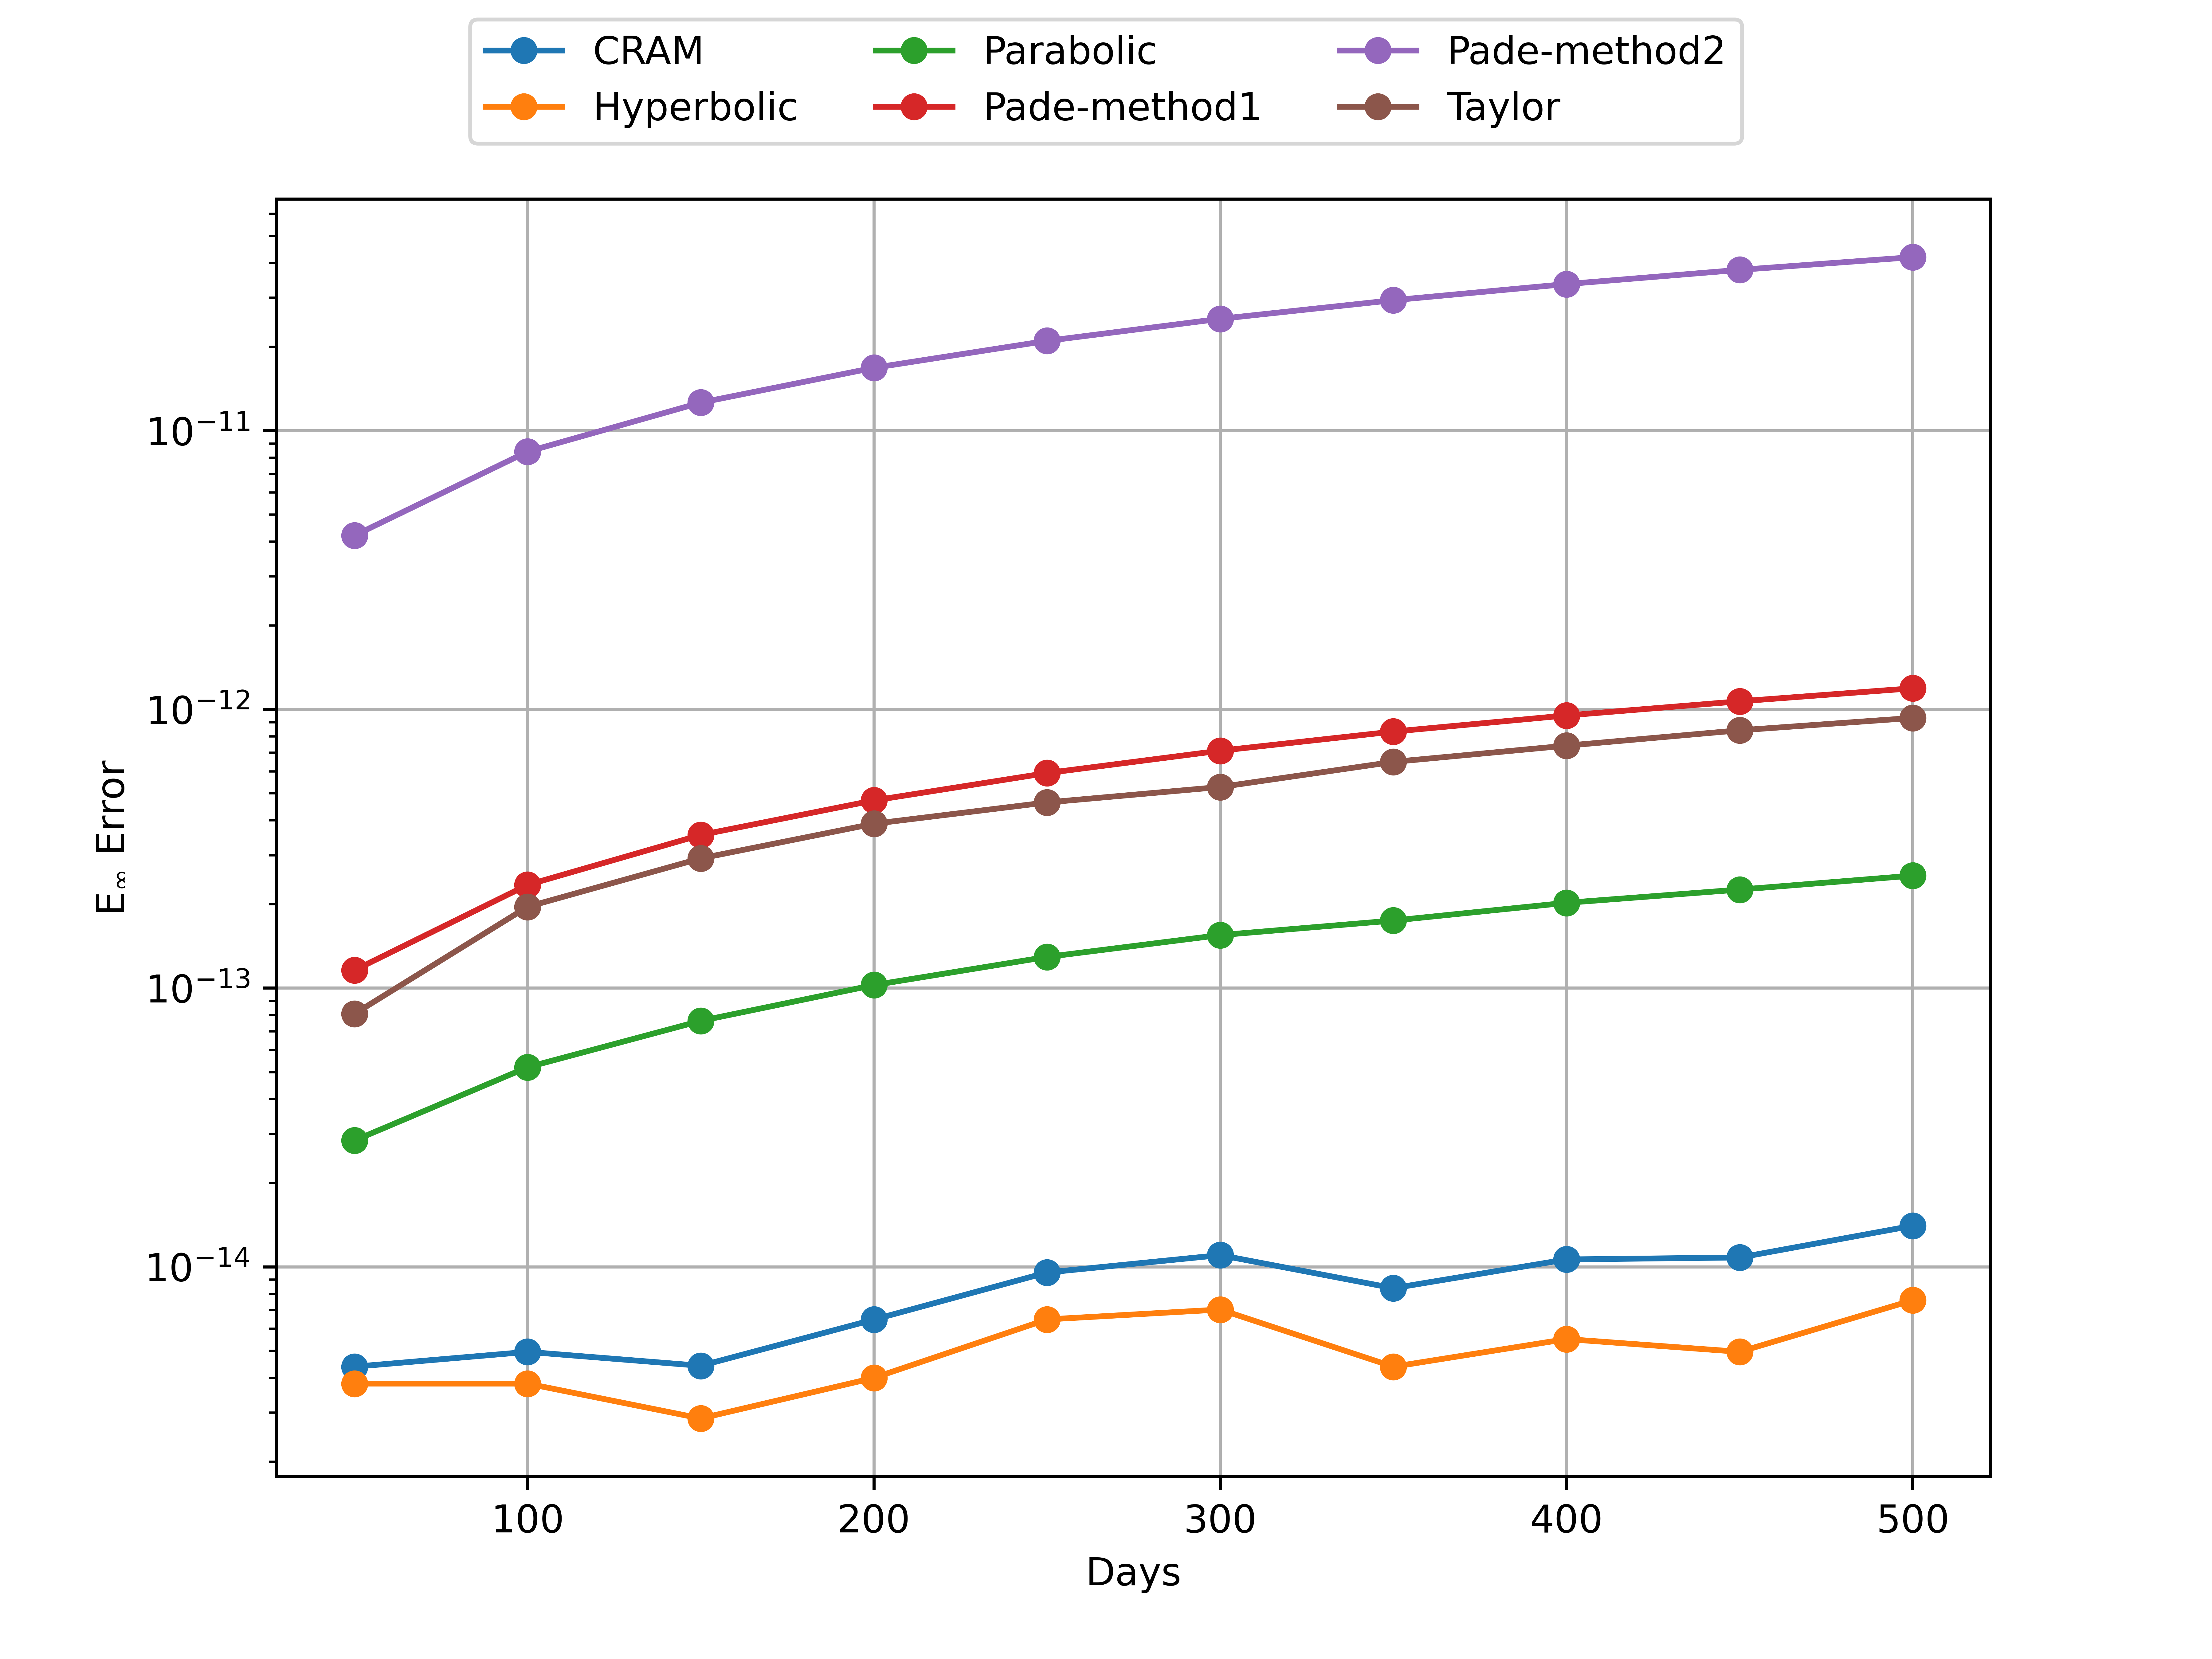
\includegraphics[width=6in]{images/chapter-5/progressionProblems/problem7/problem7EinfErrorerrorSteps4.png}
    \caption{Problem 7 E${}_{\infty}$ relative error with 4 sub-steps}
    \label{fig:problem7_Einf_error_with_steps4}
\end{figure}

\begin{figure}[p]
    \centering
    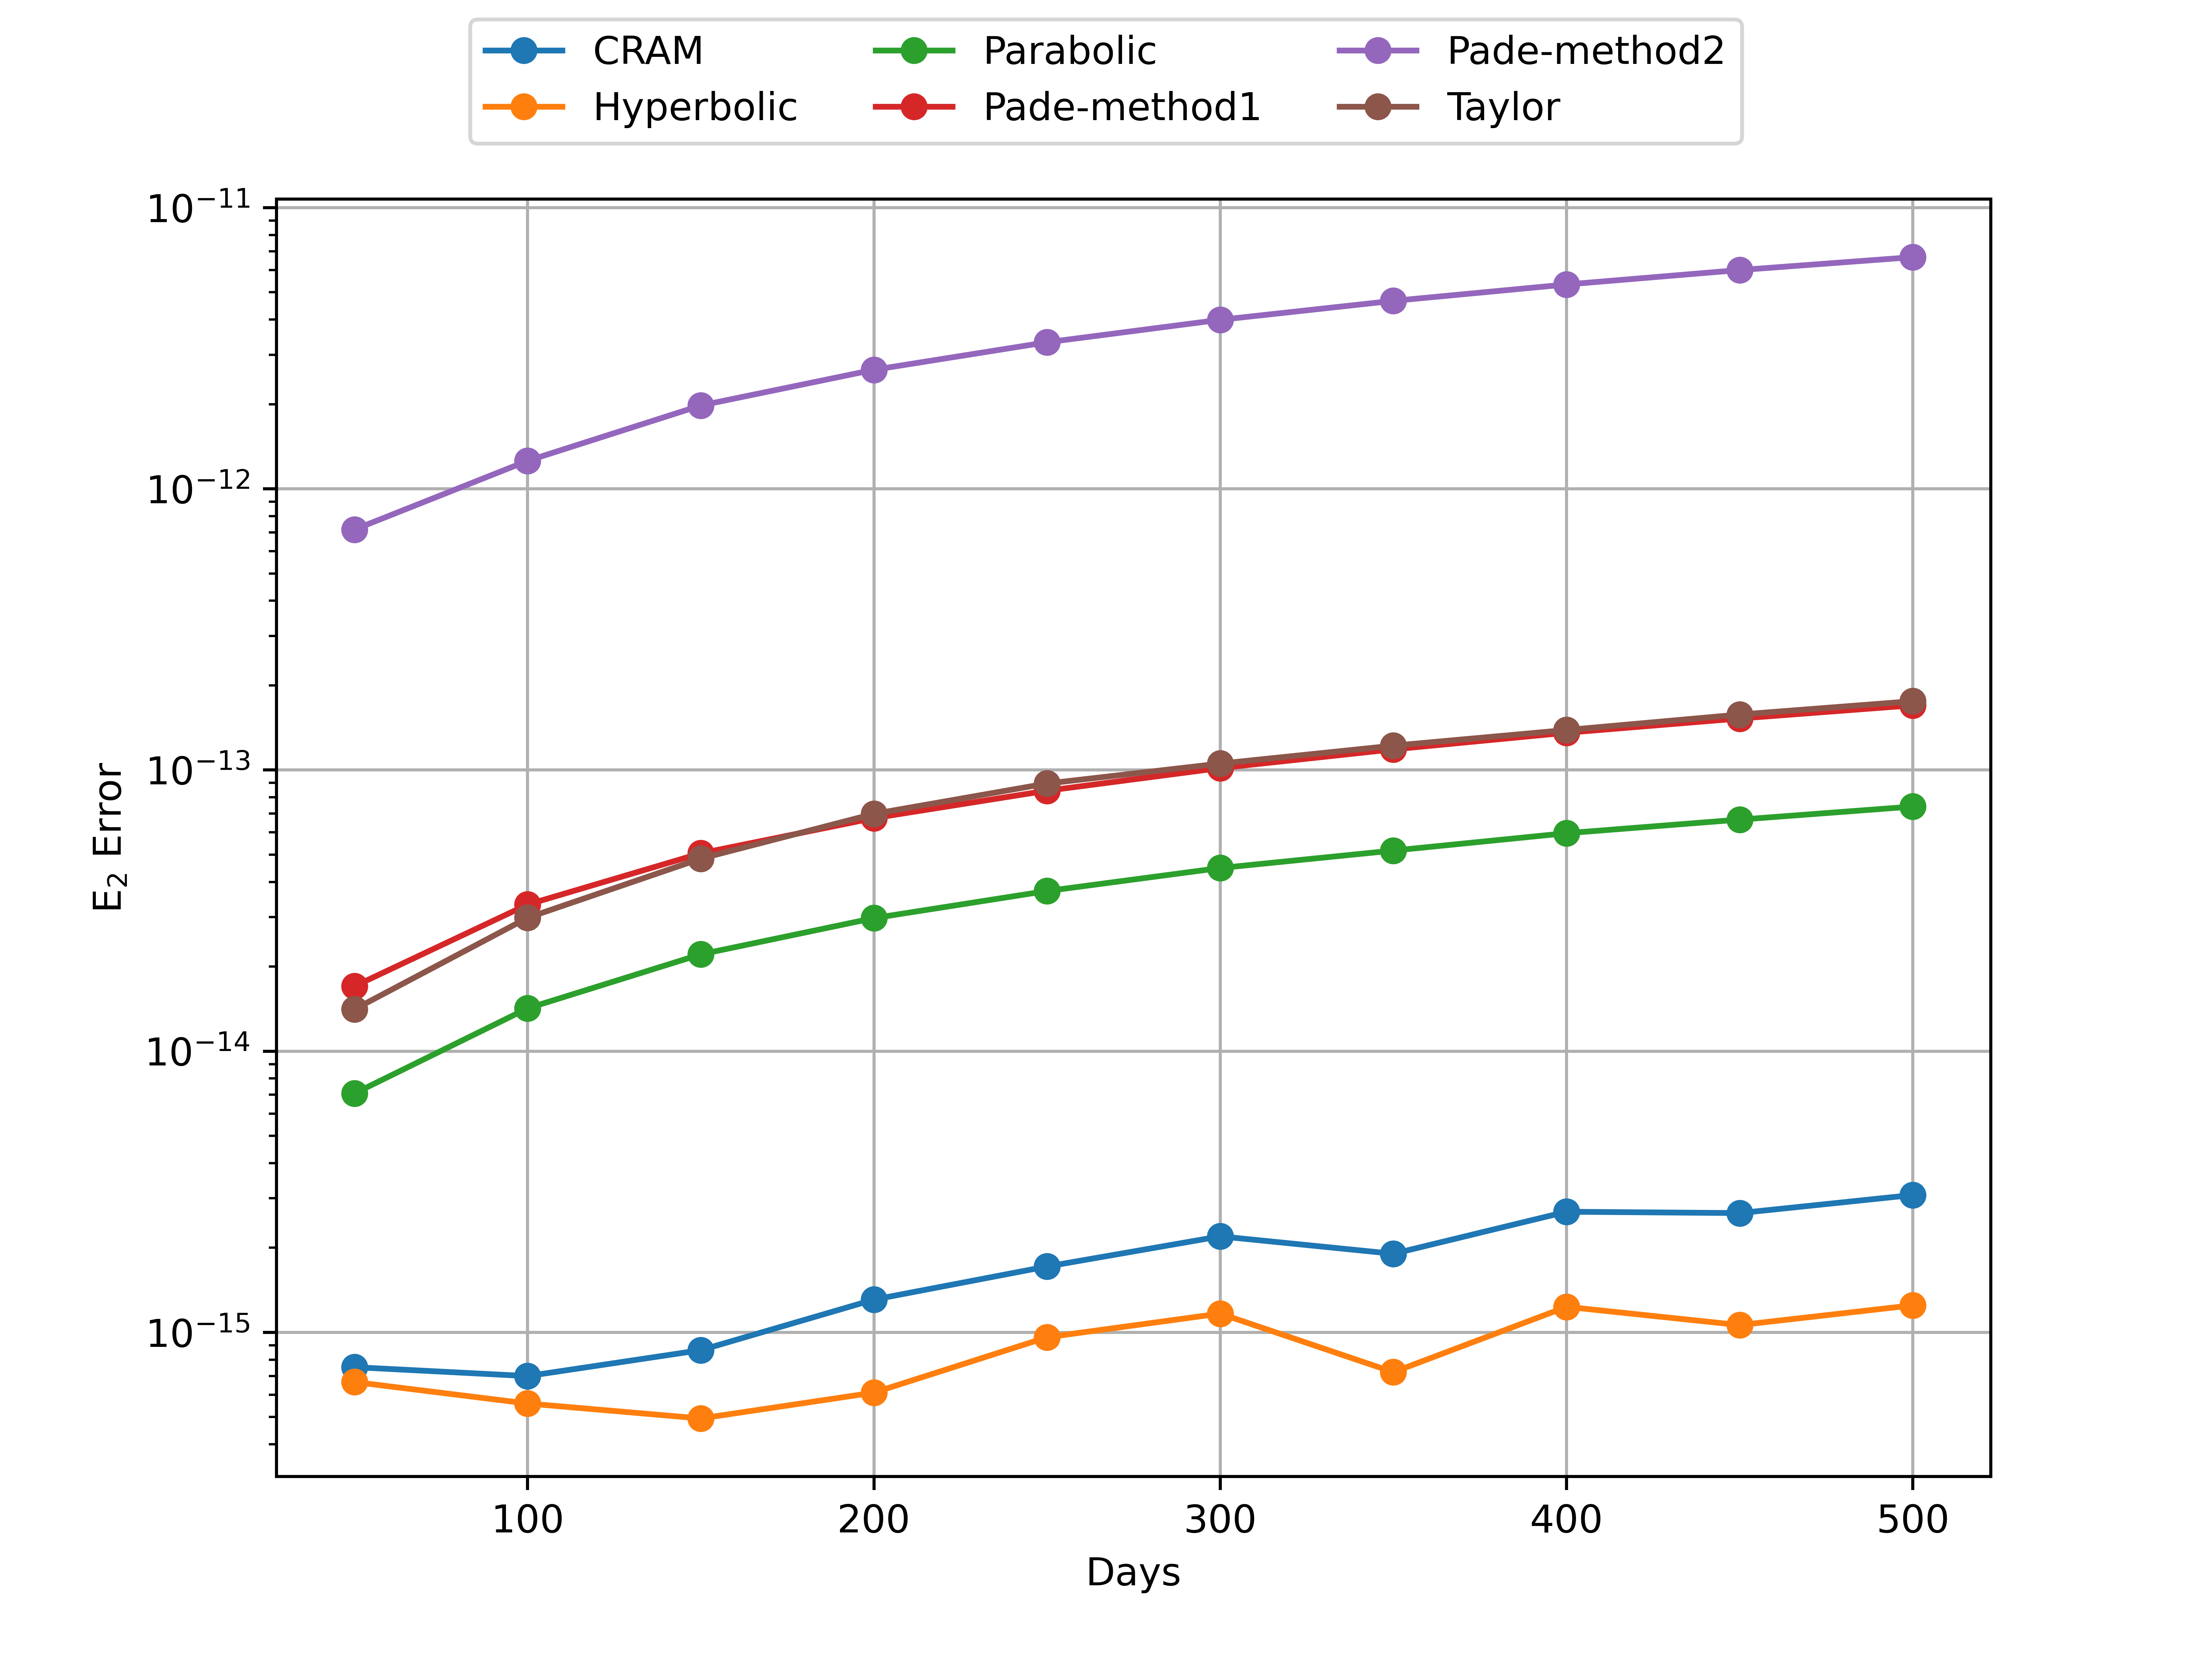
\includegraphics[width=6in]{images/chapter-5/progressionProblems/problem7/problem7E2ErrorerrorSteps4.png}
    \caption{Problem 7 E${}_{2}$ relative error with 4 sub-steps}
    \label{fig:problem7_E2_error_with_steps4}
\end{figure}

\clearpage

\subsection{Progression Problem 8}

\begin{figure}[p]
    \centering
    \includegraphics[width=6in]{images/chapter-5/progressionProblems/problem8/problem8EinfErrorWithVelocity10cells.png}
    \caption{Problem 8 E${}_{\infty}$ error with 10 cells}
    \label{fig:problem8_Einf_error_10cells}
\end{figure}

\clearpage

\begin{figure}[p]
    \centering
    \includegraphics[width=6in]{images/chapter-5/progressionProblems/problem8/problem8EinfErrorWithVelocity20cells.png}
    \caption{Problem 8 E${}_{\infty}$ error with 20 cells}
    \label{fig:problem8_Einf_error_20cells}
\end{figure}

\clearpage

\begin{figure}[p]
    \centering
    \includegraphics[width=6in]{images/chapter-5/progressionProblems/problem8/problem8EinfErrorWithVelocity40cells.png}
    \caption{Problem 8 E${}_{\infty}$ error with 40 cells}
    \label{fig:problem8_Einf_error_40cells}
\end{figure}

\begin{figure}[p]
    \centering
    \includegraphics[width=6in]{images/chapter-5/progressionProblems/problem8/problem8E2ErrorWithVelocity10cells.png}
    \caption{Problem 8 E${}_{2}$ error with 10 cells}
    \label{fig:problem8_E2_error_10cells}
\end{figure}

\clearpage

\begin{figure}[p]
    \centering
    \includegraphics[width=6in]{images/chapter-5/progressionProblems/problem8/problem8EinfErrorWithVelocity20cells.png}
    \caption{Problem 8 E${}_{2}$ error with 20 cells}
    \label{fig:problem8_E2_error_20cells}
\end{figure}

\clearpage

\begin{figure}[p]
    \centering
    \includegraphics[width=6in]{images/chapter-5/progressionProblems/problem8/problem8EinfErrorWithVelocity40cells.png}
    \caption{Problem 8 E${}_{2}$ error with 40 cells}
    \label{fig:problem8_E2_error_40cells}
\end{figure}